\documentclass[table,dvipsnames]{beamer}
\mode<presentation>{
	\usetheme{Madrid}
	\setbeamercolor{title}{fg=Black,bg=Blue!15}
	\setbeamercolor{frametitle}{fg=Black,bg=Blue!15}
	\setbeamercolor{block title}{fg=Black,bg=Blue!15}
	\setbeamercolor{block}{fg=Black,bg=Blue!10}
}

%\usepackage{default}
\usepackage{graphicx}
\usepackage{booktabs}
\usepackage{xcolor}
\usepackage{multirow}
\usepackage{minted}
\usepackage[
type={CC},
modifier={by-sa},
version={4.0},
]{doclicense}

\usepackage{tikz}
\def\checkmark{\tikz\fill[scale=0.4](0,.35) -- (.25,0) -- (1,.7) -- (.25,.15) -- cycle;} 

\definecolor{LightGray}{gray}{0.9}

\title[Devs Beginner Guide]{Basic Devs Skills for Flagship Interns}
\author{}
\date{}

\begin{document}

	\begin{frame}
	\titlepage
	\end{frame}

	\begin{frame}
		\frametitle{Disclaimer}
		\begin{exampleblock}{}
			These activities are NOT lecture or workshop activity in regular way
		\end{exampleblock}
		\begin{exampleblock}{}
			These activities are self training using prepared guideline documents 	
		\end{exampleblock}
		\begin{exampleblock}{}
			Learning by doing is the best learning way
			\begin{center}
				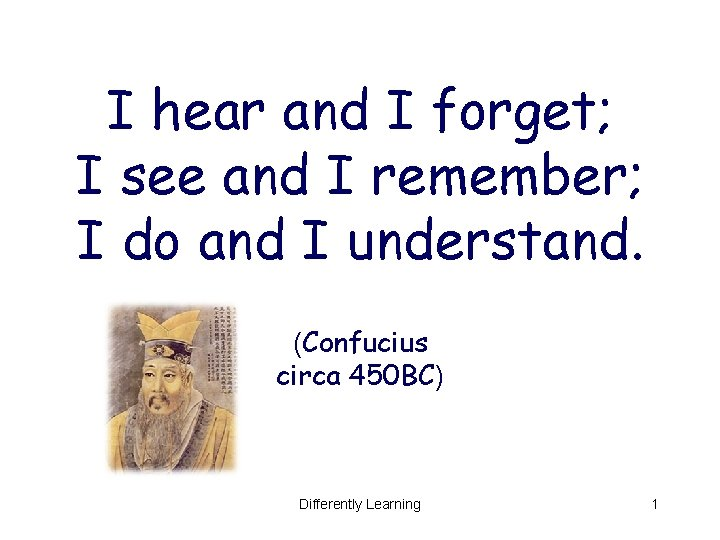
\includegraphics[width=150pt]{images/confucius}
			\end{center}
		\end{exampleblock}
	\end{frame}

	\begin{frame}
		\frametitle{Contents: Why-ies}
		\begin{exampleblock}{}
			Why need Linux ?
		\end{exampleblock}
		\begin{exampleblock}{}
			Why need Git ?
		\end{exampleblock}
		\begin{exampleblock}{}
			Why need Github ?
		\end{exampleblock}
		\begin{exampleblock}{}
			Why need Doxygen ?
		\end{exampleblock}
	\end{frame}	

	\begin{frame}
		\frametitle{Why need Linux}
		\begin{exampleblock}{}
			RaspberryPi and many single-board computer run on Linux distros
			\begin{center}
				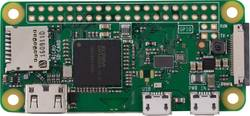
\includegraphics[width=150pt]{images/rpizerow}
			\end{center}
		\end{exampleblock}
		\begin{exampleblock}{}
			Some of popular Linux variant:
			\begin{itemize}
				\item RaspberryPi OS \\
				\url{https://www.raspberrypi.org/software/}
				
				\item Ubuntu Mate Raspberry \\
				\url{https://ubuntu-mate.org/raspberry-pi/}
				
				\item Arch Linux ARM \\
				\url{https://archlinuxarm.org/}
			\end{itemize}
		\end{exampleblock}
	\end{frame}

	\begin{frame}
		\frametitle{Why need Linux}
		\begin{exampleblock}{}
			Linux has better programming environments.
		\end{exampleblock}
		\begin{exampleblock}{}
			Some notable programming projects:
			\begin{itemize}
				\item GCC as universal C compiler.\\
				\url{https://gcc.gnu.org/}
				
				\item cross platform GUI toolkit.\\
				GTK: \url{https://www.gtk.org/}\\
				Qt: \url{https://www.qt.io/}
			\end{itemize}
		\end{exampleblock}
	\end{frame}

	\begin{frame}
		\frametitle{Why need Linux}
		\begin{exampleblock}{}
			Linux has lower hardware requirement
			\begin{center}
				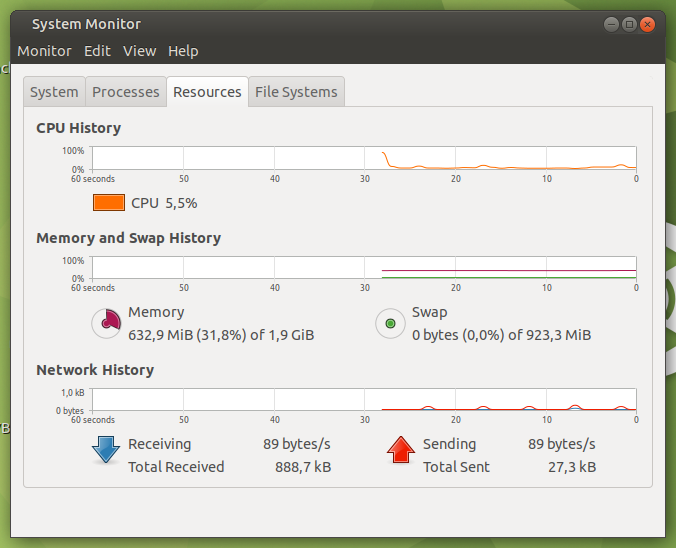
\includegraphics[width=150pt]{images/ramcpu}
			\end{center}
		\end{exampleblock}
	\end{frame}

	\begin{frame}
		\frametitle{Contents: Why-ies}
		\begin{exampleblock}{}
			Why need Linux ? \checkmark
		\end{exampleblock}
		\begin{exampleblock}{}
			Why need Git ?
		\end{exampleblock}
		\begin{exampleblock}{}
			Why need Github ?
		\end{exampleblock}
		\begin{exampleblock}{}
			Why need Doxygen ?
		\end{exampleblock}
	\end{frame}	

	\begin{frame}
		\frametitle{Why need Git}
		\begin{exampleblock}{}
			Version Control without Git in same source files
			\begin{center}
				
\includegraphics[width=250pt]{images/git_nogit}
			\end{center}
		\end{exampleblock}
		\begin{exampleblock}{}
			Version Control with Git in same source files
			\begin{center}
				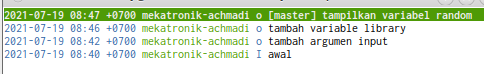
\includegraphics[width=250pt]{images/git_usegit}
			\end{center}
		\end{exampleblock}
	\end{frame}

	\begin{frame}
		\frametitle{Why need Git}
		\begin{exampleblock}{}
			Content Tracker
			\begin{center}
				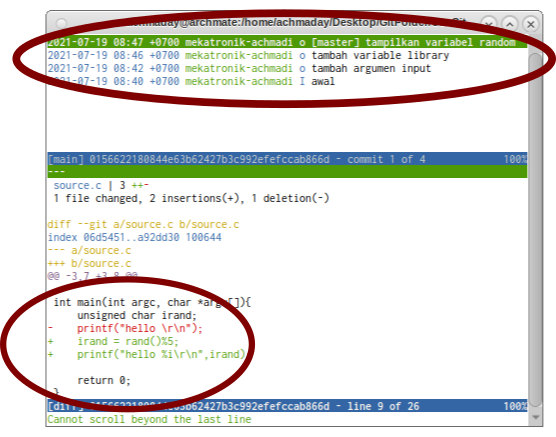
\includegraphics[width=250pt]{images/gittrack.png}
			\end{center}
		\end{exampleblock}
	\end{frame}

	\begin{frame}
		\frametitle{Contents: Why-ies}
		\begin{exampleblock}{}
			Why need Linux ? \checkmark
		\end{exampleblock}
		\begin{exampleblock}{}
			Why need Git ? \checkmark
		\end{exampleblock}
		\begin{exampleblock}{}
			Why need Github ?
		\end{exampleblock}
		\begin{exampleblock}{}
			Why need Doxygen ?
		\end{exampleblock}
	\end{frame}

	\begin{frame}
		\frametitle{Why need Github}
		\begin{exampleblock}{}
			Project Remote Storage, because:
			\begin{itemize}
				\item Google Drive is not programming friendly
				\item WhatApp is not for saving sourcecodes
				\item PasteBin only for single sourcecodes
				\item Github use Git as backend
			\end{itemize}
		\end{exampleblock}
	\end{frame}

	\begin{frame}
		\frametitle{Why need Github}
		\begin{exampleblock}{}
			Github mirror/clone of Git local:
			\begin{center}
				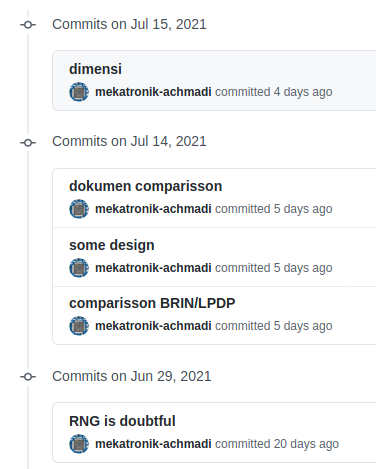
\includegraphics[width=100pt]{images/githubpiko}
				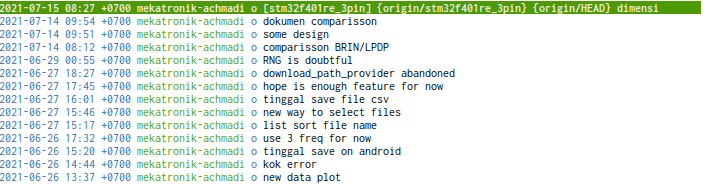
\includegraphics[width=200pt]{images/gitpiko}
			\end{center}
		\end{exampleblock}
	\end{frame}

	\begin{frame}
		\frametitle{Why need Github}
		\begin{exampleblock}{}
			Collaborative working management:
			\begin{center}
				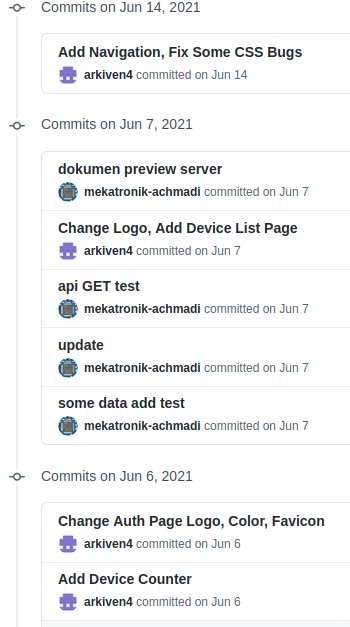
\includegraphics[width=100pt]{images/gitcollab}
			\end{center}
		\end{exampleblock}
	\end{frame}

	\begin{frame}
		\frametitle{Contents: Why-ies}
		\begin{exampleblock}{}
			Why need Linux ? \checkmark
		\end{exampleblock}
		\begin{exampleblock}{}
			Why need Git ? \checkmark
		\end{exampleblock}
		\begin{exampleblock}{}
			Why need Github ? \checkmark
		\end{exampleblock}
		\begin{exampleblock}{}
			Why need Doxygen ?
		\end{exampleblock}
	\end{frame}

	\begin{frame}
		\frametitle{Why need Doxygen}
		\begin{exampleblock}{}
			Unformatted comments:
			\begin{center}
				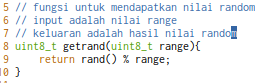
\includegraphics[width=200pt]{images/doxygenno}
			\end{center}
		\end{exampleblock}
		\begin{exampleblock}{}
			Doxygen formatted comments:
			\begin{center}
				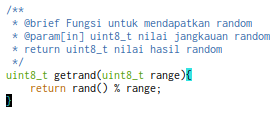
\includegraphics[width=200pt]{images/doxygenyes}
			\end{center}
		\end{exampleblock}
	\end{frame}

	\begin{frame}
		\frametitle{Why need Doxygen}
		\begin{exampleblock}{}
			HTML Doxygen result: Better Sourcecode Documentation
			\begin{center}
				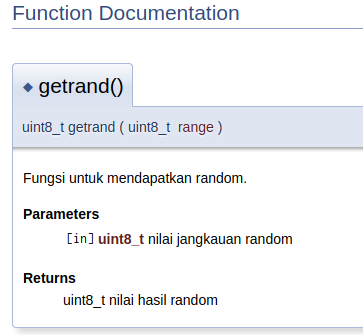
\includegraphics[width=200pt]{images/doxygen}
			\end{center}
		\end{exampleblock}
	\end{frame}

	\begin{frame}
		\frametitle{Contents: Why-ies}
		\begin{exampleblock}{}
			Why need Linux ? \checkmark
		\end{exampleblock}
		\begin{exampleblock}{}
			Why need Git ? \checkmark
		\end{exampleblock}
		\begin{exampleblock}{}
			Why need Github ? \checkmark
		\end{exampleblock}
		\begin{exampleblock}{}
			Why need Doxygen ? \checkmark
		\end{exampleblock}
	\end{frame}

	\begin{frame}
		\frametitle{Bonus: Assignment}
		\begin{exampleblock}{}
			See assignment guides here:\\
			\url{https://github.com/mekatronik-achmadi/md_tutorial/blob/master/internship/tutorials/assignment.md}
		\end{exampleblock}
		\begin{exampleblock}{}
			Some rules:
			\begin{itemize}
				\item Your assigment works will be monitored from your Github account.
				\item Drop your Github account name in max. 48 hours from now.
				\item Upload/Push your works step by step, not just final result.
				\item Do not hesitate to ask any relevant question.
			\end{itemize}
		\end{exampleblock}
	\end{frame}

\end{document}